\documentclass[spanish,12pt,letterpapper]{article}
\usepackage{babel}
\usepackage[utf8]{inputenc}
\usepackage{graphicx}
\begin{document}
	\begin{titlepage}
		\begin{center}
			
\includegraphics[width=0.6\textwidth]{../logoUnADM}~\\[1cm] 
			\textsc{Universidad Abierta y a Distancia de México}\\[0.8cm]
			\textsc{Desarrollo de Software}\\[1.8cm]
			
			\textbf{ \Large Evidencia de aprendizaje. Diseño del esquema conceptual de una base de datos.}\\[3cm]
			
			Diego Antonio Plascencia Lara\\ ES1421004131 \\[0.4cm]
			Facilitador(a): CESAR ALEXIE CHAN PUC  \\
			Materia: Diseño de Bases de Datos\\
			Grupo: DS-DDBD-1601-B1-003 \\
			Unidad: I \\
			
			\vfill México D.F\\{\today}
			
		\end{center}
	\end{titlepage}
	
	\section{Documentación del Problema}
	
	Para esta evidencia he decido resolver un problema de mi localidad y tal vez presente en muchas partes de México, este problema es referente a las pequeñas tiendas y comercios de consumo general como abarrotes, panaderías, fondas, abarrotes, tortillerías y ferreterias   pues principalmente las misceláneas y abarrotes están desapareciendo y cerrando 4 a 6 establecimientos por cada tienda de conveniencia de cadenas grandes (Oxxo, 7-Eleven, Círculo K) y mi deseo es resolver es este problema que afecta a familias de bajos recursos pues su mínimo mercado se pierde por la competencia.\\
	
Aunque aún estoy en proceso de investigación y Customer Development para conocer mas a fondo el verdadero problema y la solución que necesitan, una teoría que tengo es implementar POS para modernizar los establecimientos y aumentar la atención al cliente, las ventas y facilitar los movimientos de compra-venta e inventario a los dueños de los comercios, lo que hará un poco mas justa la competencia al poner al alcance la tecnología a estos pequeños comercios.\\

Finalmente este supuesto POS necesitara de la implementación de un sistema y una base de datos, por lo que este será mi punto de partida para la evidencia de aprendizaje, ``Base de datos para un POS''.\\

	\section{Diseño Conceptual}
	
	\subsection{Identificación de elementos}
	Al ser un punto de venta se abstrae el proceso básico de un comercio, es decir se tienen a los \textbf{Proveedores} que abastecen los \textbf{ productos} por mayoreo, estos productos son puestos a disposición del \textbf{Cliente} y entregados por una acción de compra-venta por los \textbf{Vendedores}. Lo que nos deja con la siguiente tabla:
	
	\begin{center}
	\begin{tabular}{| p{4cm} | p{4cm} |}
	\hline
	
	Entidad & Atributos\\
	\hline
	Vendedor & nombre \linebreak edad \linebreak email \linebreak numero de empleado\\
	\hline
	Cliente & nombre \linebreak edad \linebreak email \linebreak fecha y hora de registro.\\
	\hline
	Producto & nombre \linebreak precio \linebreak stock \linebreak costo\\
	\hline
	Proveedor & nombre \linebreak dirección \linebreak teléfono \linebreak email\\	
	
	\hline
	\end{tabular}
	\end{center}	 
	
	 
	\subsection{Modelo}
	
	\begin{center}
	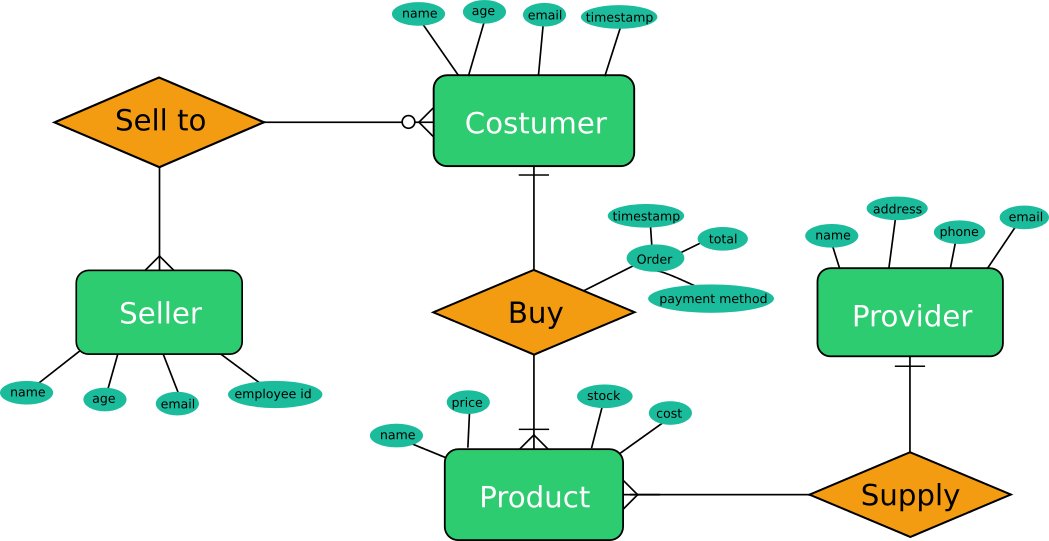
\includegraphics[width=0.8\textwidth]{./dbmodel}~\\[1cm]
	\end{center} 
	
	\section{DBMS - PostgreSQL}
	
	\subsection{Arquitectura}
	   PostgreSQL tiene una arquitectura basica de ``Proceso por usuario cliente-servidor'' y consta de un proceso demonio supervisor (postmaster), la aplicación que interactúa con el usuario, y uno o mas servidores de bases de datos (el proceso mismo de postgres).\\
	   
	   Un solo proceso Postmaster gestiona una colección dada de bases de datos en un solo host. En la aplicación del usuario la libreria libpq realiza la llamada sobre la red a Postmaster y este inicia un nuevo proceso postgres.\\
	   
	   Se puede distinguir los niveles por los recuadros, como el recuadro inferior el cual se presenta la arquitectura interna del programa que interactuá en el servidor haciendo el manejo de los datos directamente en los archivos \textbf{(nivel interior)} y en el recuadro superior la biblioteca libpg hace una abstracción para que la aplicación cliente interactúe con el servidor \textbf{(nivel externo y conceptual)}\\
	   
	   \begin{center}
	   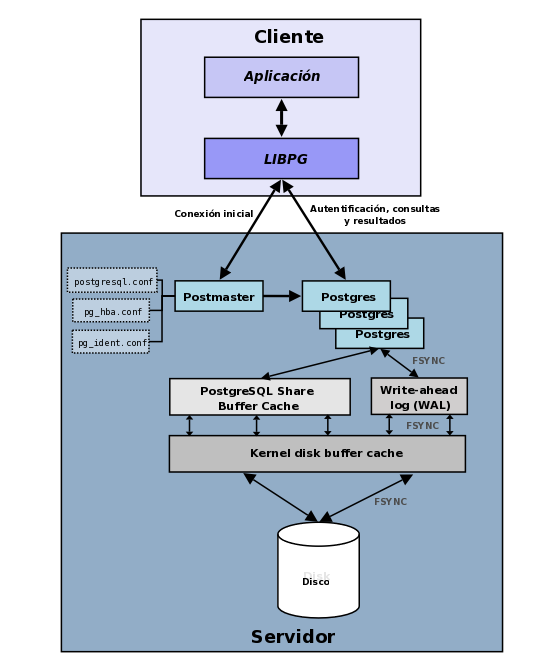
\includegraphics[width=0.5\textwidth]{./arqpq}~\\[1cm]
	   \end{center}	
	   
	   
\section{Conclusiones}

\subsection{Elección del DBMS}
Para este ejercicio seleccione PostgresSQL. Lo elegí por su licencia, que es un DBMS libre, de código abierto con licencia tipo MIT, sobre MySQL pues esta tiene licencia GPL y cuenta con licencias comerciales (requieren remuneración a Oracle); por su flexibilidad, no solo en cuanto a el código (cuenta con una librería en c), sino también por la flexibilidad en cuanto a la implementación pues permite trabajar como si fuera un RDBMS o NoSQL, e incluso un hibrido.\\

\subsection{Modelo entidad-relación}
En la imagen se observa un camino que puede comenzar desde el proveedor, esta entidad con sus datos importantes de contacto provee de los productos a precio de mayoreo a la tienda, y un proveedor puede surtir uno o mas productos. Despues uno o muchos productos cuya información permite conocer el inventario y las ganancias y datos importantes para la venta (precio-costo), son adquiridos por un solo cliente en una transacción de compra-venta. Al comprar el cliente se establece un vinculo cliente-vendedor el cual queda registrado así como queda registrada la venta con los datos de la orden y los datos del cliente y vendedor.

\subsection{Dificultades}
Lo que se me dificulto mas fue al momento de realizar el modelo entidad-relación pues había cierta confusión al momento de definir los tipos de relaciones, pues había que tener en mente solo el momento de una transacción pues hubo momentos donde lo olvidaba y tenia en mente mas de una transacción lo que hubiera terminado en puras relaciones muchos a muchos.
	
	\pagebreak
	\begin{thebibliography}{9}
	\bibitem{economiahoy} Economía Hoy México. 
		\emph{Oxxo triunfa en el sector de las cadenas de ventas de conveniencia}. Economía Hoy, [Disponible en: http://www.economiahoy.mx/empresas-eAm-mexico/noticias/6861986/07/15/Oxxo-triunfa-en-el-sector-de-las-cadenas-de-ventas-de-conveniencia.html].
		
		\bibitem{rrhopkins} Robert J. Robbins. 
		\emph{Database Fundamentals}. Johns Hopkins University, [Disponible en: http://www.esp.org/db-fund.pdf].
		
		\bibitem{elmasriynavathe} Ramez Elmasri and Shamkant Navathe. 
		\emph{Fundamentals of Database Systems}. Pearson Education, [Disponible en: http://tinman.cs.gsu.edu/~raj/4710/f11/Ch01.pdf].
		
		\bibitem{psqldocs} The PostgreSQL Development Team. 
		\emph{PostgreSQL 7.0 Docs}. PostgreSQL, [Disponible en: http://www.postgresql.org/docs/7.0/static/postgres.htm].
		

	\end{thebibliography}

\end{document}